\chapter{Guidelines}\label{chapter:guidelines}
\section{Context}\label{section:guidelines/context}
The major objective of the research is to devise some guidelines so that the task of approaching any complex problem domain using microservices becomes easier. On the way to that, a few research questions related to various crucial topics on microservices emerged. The research questions were taken as stepping stones for discovering guidelines. The topics are already covered in previous chapters. 
\\
At first, the concept related to granularity of microservices is studied in detail in Chapter \ref{chapter:granularity}. In this chapter, the semantic meaning of size along with various dimensions defining granularity are discussed. Finally, various principles to help find the optimum size for microservices are listed.
\\
Secondly, other quality attributes to be considered when designing good microservices were listed in Chapter \ref{chapter:quality_of_service}. The quality metrics to determine each of these quality attributes are also mentioned. The various quality metrics lead to a limited list of basic metrics. Finally, various principles to determine quality of good services along with the way the quality attributes affect each other are recorded.
\\
Next, the ways to decompose problem domain in order to identify microservices are discussed in Chapter \ref{chapter:service_candidate}. The methods discussed are using domain driven design and use case refactoring. The steps involved in each method are described along with an example.
\\
Till then, answers related to granularity , quality attributes and process of identifying microservices are derived from literature. In Chapter \ref{chapter:hybris_architecture} attempt is made to find answeres from industry experience by studying the architecture at SAP Hybris and conducting various interviews. With the knowledge, series of steps are shown to visualize the process of breaking down problem domain into microservices.
\\
Finally, the challenges which come up while implementing microservices architecture are discussed in Chapter \ref{chapter:challanges_of_microservices_architecture}. In this chapter, various ways to tackle these problems are described.

\section{Process to Implement Microservices Architecture}\label{section:guidelines/process_to_microservices}
As shown in the Figure \ref{fig:guidelines/chapter_nine_process}, the implementation of microservices consists of two major parts, understanding each part is crucial in order to follow microservices architecture.
\begin{enumerate}
\item \textbf{modeling microservices} \\
The core of the microservices architecture is problem domain and understanding it. Modeling microservices divides the problem domain into various components considering various internal quality attributes such as coupling, cohesion etc. The knowledge regarding quality attributes acts as an input when choosing the efficient process for identifying microservices from problem domain.
\item \textbf{operating the microservices artifacts in production environment} \\
The way microservices are designed to satisfy various external quality attributes such as scalability, resilience etc. However, it also introduces critical challenges. It is not entirely possible to get the advantages from microservices architecture unless these challenges are identified and tackled appropriately. In order to achieve that, certain implementation and operational practices of microservices need to be followed.
\end{enumerate}
\begin{figure}[H]
\begin{center}
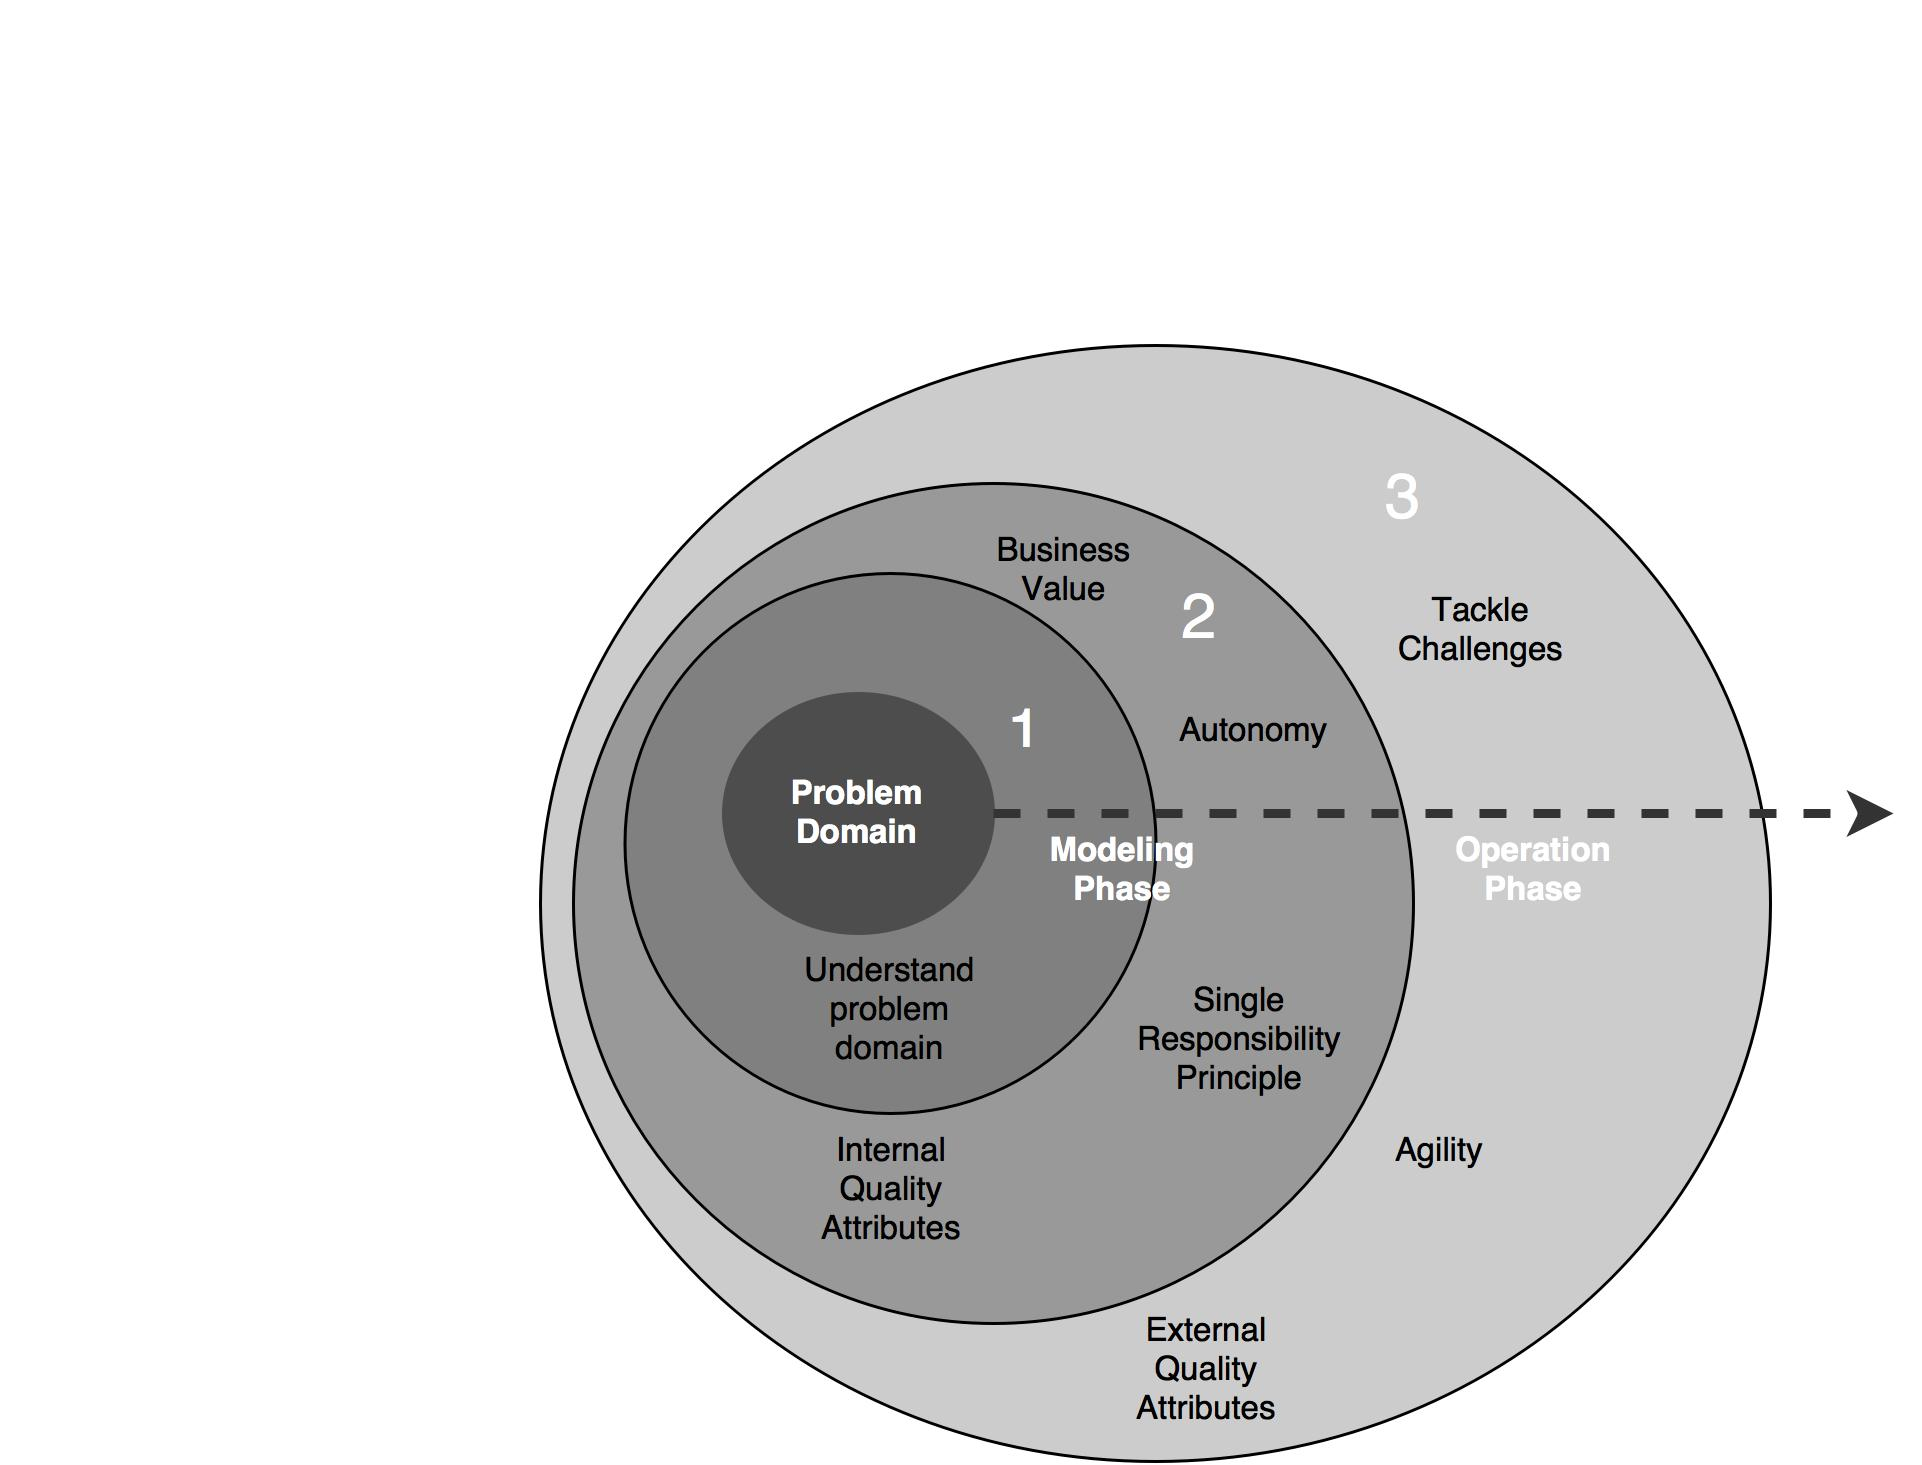
\includegraphics[width=0.7\textwidth]{figures/chapter_nine_process}
\caption{Process to implement microservices architecture}
\label{fig:guidelines/chapter_nine_process}
\end{center}
\end{figure}
\\
The microservices architecture follows a process which guides from understanding the problem domain, identifying modular components considering various attributes, implementing and operating the components to satisfy various external quality attributes. It is interesting to find how process, principles and guidelines are related. A process is based upon some basic principles whereas principles helps to define guidelines based upon some specific requiement and environment. So, in order to understand the process of implementing microservices, it can be helpful to look into some broad basic principles.

\section{Principles And Guidelines}\label{section:guidelines/principles_and_guidelines}
In this section, based upon the research findings as discussed in previous chapters, various principles are presented in order to tackle modeling microservices as well as operating them in release environment. It is highly recommended to follow these principles when considering microservices.\cite{Newman:2015aa}
\begin{enumerate}
\item \textbf{Correct Granularity} \\
The dimension of granularity for microservice is given by functionality it performs, data it handles and business value it provides. \ref{section:granularity/dimensions} These dimensions make it pretty obvious how to make the size of a service as low as possible. However, the notion of correct granularity is rather important and should be only focus instead of attempting to make the size lowest possible.\ref{section:granularity/principles} There are various factors which act together and tailor the size of microservice.
\begin{enumerate}
\item One of the factors is \textbf{\acrshort{SRP}}, which influence the functionalities and data handled by microservices to make it as small as possible. \acrshort{SRP} encourages to focus on small set of cohesive tasks which change for same reason. \cite{Stine:2014aa} \cite{Newman:2015aa} The influence of \acrshort{SRP} on is also verified by the result of interview which is compiled in Section \ref{section:hybris_architecture/interview/interview_compilation}.
\item Another important factor is \textbf{autonomy}. According to S. Newman, a microservice should be able to be deployed and updated independently. \cite{Newman:2015aa} Without any surprise, autonomy is an important quality attribute of microservice and is evaluated as the degree of control upon operations to act on its business entities only. \ref{section:quality_of_service/quality_metrics/autonomy} As discussed in Section \ref{section:granularity/principles}, a microservice should provide transaction integrity such that it is big enough to support activities which fall under one transaction. So, autonomy tends to limit the scope of functionality and data such that the service is self-contained, self-controlling and can be self-governed.\cite{Ma:2007aa}
\item The act of realizing the size of microservices as small as possible comes with a price. As the functionality of microservice is squeezed, the number of microservices needed for any application increases. The task of deploying, provisioning and governing these microservices can be challenging. So, as stated in the principles defined in Section  \ref{principle:granularity/IT_infrastructure},  the decision regarding the size of service should be rational based upon the current \textbf{infrastructure and operational capability} to handle such large number of small microservices. It is further supported by the response of interview compilation in Section \ref{section:hybris_architecture/interview/interview_compilation}
\item Finally, the size of microservices according to functionality and data should also relate to ultimate \textbf{business value} and should coincide with the business goal. It is also evident from the response of interview compiled in Section \ref{section:hybris_architecture/interview/interview_compilation}. Additionally, business value being an important dimension of granularity of microservice according to Section \ref{section:granularity/dimensions}, should be examined before choosing the functionality being performed by a service.
\end{enumerate}
So, while deciding about the size of microservice the mentioned factors should be well considered.

\item \textbf{Consider quality attributes as early as possible} \\
The internal quality attributes such as coupling, cohesion, autonomy etc should be controlled as early as possible during modeling and development phases. Taking care of the internal qualities will eventually help to control the external qualities of the microservices in release such as reusability, reliability, resilience etc. The Table \ref{tab:quality_of_service/quality_attributes/basic_quality_metrics} which identifies various attributes in terms of basic metrics can be helpful. For one thing, the metrics such as scope of opertions, number of operations used in the basic metrics table are completely in disposal of the developers and teams of microservices. Secondly, it helps to identify the relationship among them as shown in Table \ref{tab:quality_of_service/quality_attributes/quality_attributes_relationship} which assists in managing trade offs needed.

\item \textbf{Understand the problem domain}\\
As discussed in chapters , problem domain can be analyzed using either usecase modeling or domain driven design. \\
Using usecase can break down the problem domain into level of abstractions, each abstraction representing lower scope of functionality. The graphical approach used in usecase can be an effective approach in brainstorming and exploring the problem domain to find new usecases.\\
Another popular approach is using domain driven design to explore problem domain. The overall process looks natural and straight forward which focus on dividing the complex domain into manageable subdomains and further into modular autonomous components. Furthermore, it gives emphasis on using ubiquitous language to find modules and define their boundaries. The chapter provides important guidelines as well as hints on ubiquitous language and to find bounded contexts.\\
Although the graphical approach provided by usecases are wellsuited to experience and can be faster, but they tend to focus only on \acrshort{SRP} and scope of functionality. Following the process may likely lose grip on very important quality attribute of microservices which is autonomy.\\
Domain driven design on the other hand, with its approach of using ubiquitous language focus on autonomy and by dividing the problem domain into smaller manageable components also focus on autonomy. Although the whole proces seems natural, getting the boundary right is complex process. A clear understanding of the problem domain is necessary to get the bounded context right. So, it can be an iterative process starting at bigger boundaries at first and then down to smaller modular boundaries in several iterations.\\
The knowledge and practice of both usecase modeling and domain driven desing can be helpful. Depending upon the complexity of the problem domain and experience with it, any of them or combination of them can be used to understand the problem domain well.

\item \textbf{Culture of Automation}\\
With such a large number of small services, the task of managing and operating them manually can become impossible. There are three specific areas where automation can serve greatly.
\begin{enumerate}
\item Automated Continuous Delivery can help building and deploying microservices frequently with consistency. Maintaining continuous integration and delivery pipeline can make sure that any new changes is consistent to old system and can be put into release in a matter of few button presses.
\item Automated Testing is another important area to be serious when there are large number of microservices and again large number of changes in the backlog. Without automated testing in sync with delivery pipeline, it can be hard to have confidence of deploying changes to release environment without breaking existing functionalities.
\item Infrastructure Automation and Provisioning should not be neglected, especially when there can be different technology stack in different microservices and different infrastructure environments. \acrshort{PaaS} such as CloudFoundry can be helpful to deployment and provision easily whereas various configuration management tools such as Puppet, chef etc can assist to manage different technology stacks.
\end{enumerate}
\item \textbf{Hide Internal Implementation}\\
Collaboration among microservices is essential however high coupling by over exposing inner details should be avoided to save autonomy.
\begin{enumerate}
\item The first on the checklist is to model the \acrshort{API}s in right way. Rather than breaking the application into technological aspects, the problem domain should be clearly understood to discover clear boundaries and so should be modeled around business domains. The concept of bounded context can be a way to define clear \acrshort{API}s reducing unnecessary coupling.
\item The \acrshort{API}s should be technology agnostic, which means that the technology used for collaborating between \acrshort{API}s should not guide the implementation of them. Using \acrshort{REST} and some form of \acrshort{RPC} can help to tackle them.
\item In microservices, database is also an integral part of internal implementation. Already mentioned in Section \ref{section:challanges_of_microservices_architecture/integration/sharing_data}, sharing database will tightly couple microservices as it exposes internal data structure details. In order to solve that each microservice should atleast have its own private tables or schema per each service or at most separate database server.
\item Additionally, in order to maintain loose coupling, the integration technology should be well thought. As already discussed in Section \ref{section:challanges_of_microservices_architecture/integration/inter_service_communication}, if business requirement allows, asynchronous communication styles such as publish/subscribe, notification, request/async response should be chosen over synchronous request/response.
\end{enumerate}
\item \textbf{Decentralize} \\
Autonomy should not be limited to deployment and updates only. It should be applied in team organization as well. A team should be autonomous enough to own services completely from developing the microservices, releasing them and maintaining in the production environment all by themselves. In order to achieve that, teams should be trained to become domain-experts in the business areas which are focussed by their services.
Additionaly, the architecture of microservices should follow decentralization as well. The business logic should be divided among microservices and should not be concentrated towards any specific god services and integration mechanism. With that point, the microservices should be smart enough to handle collaboration among themselves and the communication mechanism should be dumb as possible such as \acrshort{REST} and messaging. Also, choreography should be highly applied whenever possible and orchestration should only be used if the business requirement dictates so.
\item \textbf{Deploy Independently}\\
Microservices should be able to be deployed independently. The Section \ref{section:challanges_of_microservices_architecture/integration/breaking_change} already discusses the challenges for that as well as solutions.
\begin{enumerate}
\item In order to avoid breaking changes, an integration technology such as \acrshort{REST} should be used to decouple microservices and tollerant reader pattern should be used to implement consumers.
\item To find the breaking changes early during development, consumer-driven contracts should be implemented as automated test in the delivery pipeline of services. Additionally, semantic versioning can be used to clearly indicate the level of new changes.
\item When breaking changes cannot be avoided, maintaining co-existing endpoints of different versions or co-existing service versions can provide enough time and opportunity to consumers to be updated gracefully without breaking \acrshort{API}s.
\item Finally, the release and deployment can be decoupled using techniques such as bluegreen deployment \ref{section:appendices/blue_green_deployment} and canary release \ref{section:appendices/canary_release}, so that new changes can be tested in production with confidence and can be released later to reduce the risk.
\end{enumerate}
\item \textbf{Consumer First}\\
Microservices are made in order to serve its consumers, so consumers should be the priority when designing them.
\begin{enumerate}
\item \acrshort{API}s should be designed considering its consumers. It should be easy to understand, use and extend. The name as well as link should be self intuitive. Additionally, documentation should be provided which should be helpful to follow and use \acrshort{API}. In order help with these, there are various tools available such as swagger, RAML etc. The tools not only make it easy to design and document \acrshort{API}s but also enable to try them.\cite{Bloch:2016aa} \cite{Blanchette:2008aa}
\item Another important concept is to make it easy for consumers to find the microservice itself. There are various service discovery tools such as zookeeper, etcd, consul etc which can be used.
\end{enumerate}
\item \textbf{Isolate Failures}\\
Microservices are build on the top of distributed system and it is not false to say they are not reliable.\cite{Factor:2014aa} With the consent of amount of microservices and collaboration among them, the system should not be affected until all the microservices fail. The solutions are discussed in Section \ref{section:challanges_of_microservices_architecture/handling_failures}.
\begin{enumerate}
\item Timeout should be implemented realizing the fact that remote calls are different than local calls and they can be slow. A realistic value of timeout should be chosen based on the use case scenario.
\item In order to avoid leaking failures and affecting the whole system as a result, bulkhead should be used to segregate the resources and a thereshold value should be maintained for each group of resources.
\item For reducing latency, circuit breaker should be implemented which detaches a failed node after certain attempts and reattemts automatically. In this way, it not only removes unnecessary roundtrip time or waiting time but also saves network resource.
\item Finally, fallback mechanism can be used in conjunction with timeouts and circuit breaker to provide alternative mechanism such as serving from cache. It not only isolates failure but also serves the request.
\end{enumerate}
\item \textbf{Highly Observable} \\
It can be difficult to observe the status of each microservice on each provisioned hosts considering the number of microservices. The Section \ref{section:challanges_of_microservices_architecture/monitoring} points out some ideas which can be used to make it easier.
\begin{enumerate}
\item Use semantic monitoring to check the current behaviour of services such as availability, response time etc. An example of tools to accomplish that is uptime. Additionally, trigger certain tests to verify important logic of microservice in regular basis. One way to achieve that is to trigger smoke tests automatically.
\item In order to get the overall picture of the whole application at one place, use logs aggregation and visualization tools such as logstash and kibana.
\item Finally, use correlation ids to get a semantic picture of related requests branched out along many downstream microservices.
\end{enumerate}
\end{enumerate}